\input{texheder.tex}
\usepackage{setspace} % setspaceパッケージのインクルード
\usepackage{enumitem}
\usepackage{graphicx}
\usepackage{grffile}
\usepackage{url}

%「Weekly Report」
\newcommand{\Weekly}[5]{
\twocolumn[
    \begin{center}
    \bf
    第 #1 回 Weekly Report\\
    \huge
    スマートフォンのスイング動作に潜在する個人特性\\
    \LARGE
    --- フルフルによる個人認証 ---\\

    \end{center}
    \begin{flushright}
        #2 月\ \ \  #3 日 \ \ \ #4 \
        #5
    \end{flushright}
    ]
}
%\setstretch{0.5} % ページ全体の行間を設定

\begin{document}

\Weekly{2}{4}{20}{(火)}{\ 中島 基晴}


%%%%%%%%%%%%%%%%%%%%%%%%%%%%%%%%%%%%%%%%%%%%%%%%%%%%%%%%%%%%%%%%%%%%%%%%%%%%%%%%%%%%%%%%%%%%%%%%%%%%%%%%%%%%%%%%%%
%%%%%%%%%%%%%%%%%%%%%%%%%%%%%%%%%%%%%%%%%%%%%%%%%%%%%%%%%%%%%%%%%%%%%%%%%%%%%%%%%%%%%%%%%%%%%%%%%%%%%%%%%%%%%%%%%%
\section{今週までの作業内容}
\begin{itemize}
    \item 移動平均法の決定.

    先週の課題に挙げていた3つの移動平均法のうち,荷重移動平均法を決定した.
    
    \item 正規化をせずに検定を行う.
    
    正規化を行うと個人特性が失われるので正規かは行わない.

    \item 等分散性の検定を行った.
    
    母平均の差の検定では母分散が等しいと仮定して検定を行う.
    等分散性の検定はこの裏付けをとるために行う.母分散が
    等しいという仮説が棄却されなければ,母分散が等しいことを
    積極的に捨てる根拠が弱いと判断できる.

    \item ある2人のデータの検定結果の報告.
    
    先週で今秋までの課題に挙げたある2人のデータの検定結果が
    出たので報告する.
\end{itemize}

この4つの項目のうち,移動平均法の決定,等分散性の検定結果,
ある2人のデータの検定結果を詳しく述べる.
%%%%%%%%%%%%%%%%%%%%%%%%%%%%%%%%%%%%%%%%%%%%%%%%%%%%%%%%%%%%%
\section{移動平均法の決定}

\subsection{単純移動平均法}

先週では式\ref{eq:simple_1}と式\ref{eq:simple_2}を紹介した

\begin{equation}
    Y(k) = \frac{1}{n + 1}\sum_{i=-n}^{0}A(k + i)
    \label{eq:simple_1}
\end{equation}

\begin{equation}
    Y(k) = \frac{1}{2n + 1}\sum_{i=-n}^{n}A(k + i)
    \label{eq:simple_2}
\end{equation}

式\ref{eq:simple_1}は$k$番目のデータとそれより前の$n$個のデータとの
平均を取り,式\ref{eq:simple_2}は$k$番目のデータとその前後にある$n$個のデータとの
平均を取る式である.
その時に式\ref{eq:simple_1}を使用すると述べたが,
Python では式\ref{eq:simple_2}にすることができると知ったので
これからは式\ref{eq:simple_2}を用いることにした.
式\ref{eq:simple_1}では平均後のグラフがもとのグラフとずれるので,
比較する時にグラフを一致させる作業が必要であった.
しかし式\ref{eq:simple_2}を使用すると個のずれがなくなるので
グラフを一致させる作業を省くことができる.

次に荷重移動平均法と指数移動平均法の説明を先週に行っていなかったので説明する.

%%%%%%%%%%%%%%%%%%%%%%%%%%%%%%%%%%%%%%%%%%%%%%%%%%%%%%%%%%%%%
\subsection{荷重移動平均法}

荷重移動平均法は,過去のデータになるに取れて重みを
線形的に減少させる手法である.
例えば$5$つのデータで加重平均を行う場合,$k$番目のデータの重みは$5$,
$k - 1$番目のデータの重みは$4$,そして$k - 4$番目のデータの重みは$0$になる.
加重平均方法の式を式\ref{eq:kaju_average}に定義する.

\begin{equation}
    W(k) = \frac{\sum_{i=1}^{n}(i \times A(k - n + i))}{\sum_{i = 1}^{n}i}
    \label{eq:kaju_average}
\end{equation}
これは$k$番目ののデータを$A(k)$,$k$番目の演算結果を$W(k)$とする.但し,$k \geg n$である.
$k$番目のデータから$A(k - n + 1)$に対して線形的に重みを減らしていき,それらの和を
重みの合計値で割ることで$W(k)$を求めることができる.

%%%%%%%%%%%%%%%%%%%%%%%%%%%%%%%%%%%%%%%%%%%%%%%%%%%%%%%%%%%%%
\subsection{指数移動平均法}

指数移動平均法は,過去のデータになるについて重みを指数的に減少させる手法である.
重みのレベルは平滑化係数$\alpha$によって決定され$0 \sim 1$の範囲で値を取る.
一般的に$N$個のデータに対して指数移動平均法を用いる時,式\ref{eq:keisu}
で平滑化係数$\alpha$を決定する.

\begin{equation}
    \alpha = \frac{2}{N + 1}
    \label{eq:keisu}
\end{equation}
また,指数移動平均法を式\ref{eq:sisu_average}で定義する.

\begin{equation}
    E(k) = \alpha A(k - 1) + (1 - \alpha)E(k - 1)
    \label{eq:sisu_average}
\end{equation}

$k$番目のデータを$A(k)$,$k$番目の演算結果を$E(k)$とする.
但し,$k \geq 3$である.直前のデータを$A(k - 1)$と直前のデータに対して
指数移動平均法を行った$E(k - 1)$を$(1- \alpha)$倍した値の和が$k$番目の
指数移動平均の結果となる.

%%%%%%%%%%%%%%%%%%%%%%%%%%%%%%%%%%%%%%%%%%%%%%%%%%%%%%%%%%%%%
\subsection{評価方法}

これら3種類の移動平均法から適切な手法を決定する方法として,
図\ref{fig:average}のように,
以前にある2人から得た$x$成分,$y$成分,$z$成分の加速度,そして
絶対加速度の計4種類のデータに対してそれぞれの移動平均法を適用した.

\begin{figure}[tb]
    % \centering
    \vspace{-50mm}
    \hspace{0.3cm}
    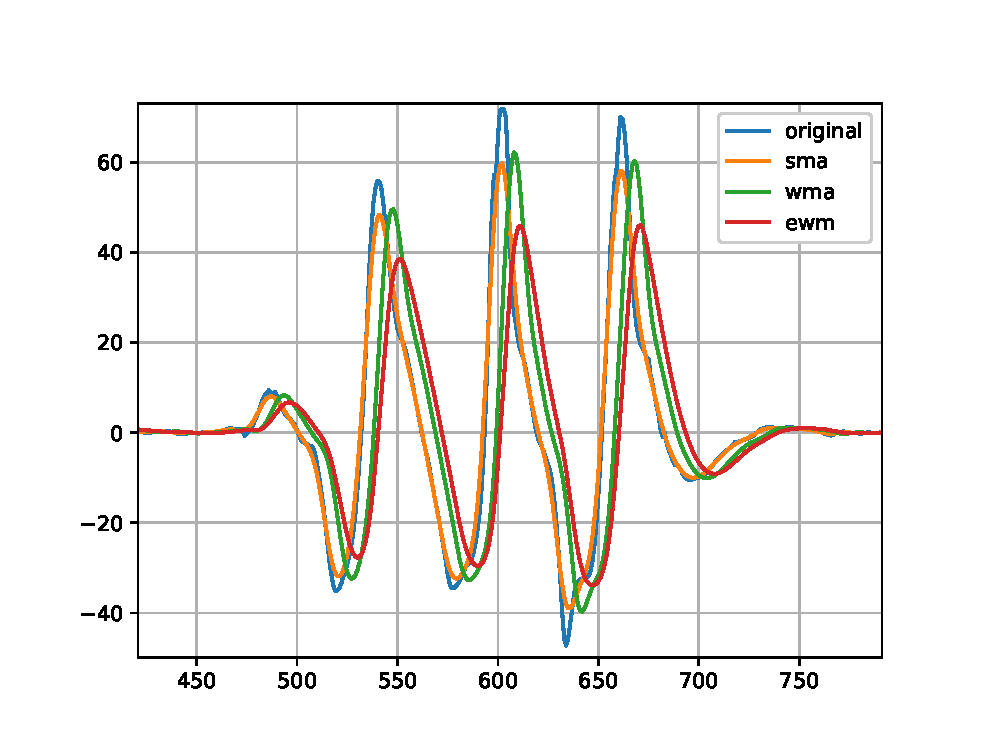
\includegraphics[scale=0.6]{images_S2/KP2_20210416_average.eps}
    \vspace{35mm}
    \hspace{-3.5cm}
    \caption{移動平均後処理前後の比較}
    \label{fig:average}
\end{figure}


2人からそれぞれ3回分の計測データを得たので,$2 \times 3 \times 6 = 24$個の
評価結果を得られる.
青色のグラフが処理前のデータ(original),黄色のグラフが単純移動平均(sma),
緑色のグラフが加重移動平均(wma),赤色のグラフが指数移動平均(ewm)である.
また,平均を取る範囲を$n = 5$,試行回数を5回とした.ここで試行回数とは,
移動平均を処理した回数のことである.
試行回数1回の場合は処理前のデータに移動平均処理を1回行う.2回の場合は
1回処理したデータに再び移動平均処理を行う.
各移動平均の評価方法として,Pythonの機械学習ライブラリの scikit-learn に
ある計算メソッド sklearn.metrics.r2_score を用いる.
これは決定係数$R^2$というモデルの当てはまりの良さを示す指標で,
最も当てはまる場合,$1.0$ となる.
この決定係数が最も大きい移動平均法を採用とする.❝sma❞,❝wma❞,❝ewm❞ のうち,
最も決定係数が高い手法を$1$,それ以外を$0$ として24個の評価結果を
表\ref{table:evaluation}に示す.

すべての結果において加重平均方法が他の移動平均法と比較して優れているという結果になった.
更にグラフから,十分な平滑化ができていると考えることができる.
以上より本研究では加重平均方法を用いてノイズの除去を行う.

\begin{table}[tb]
    \caption{各移動平均の評価結果}
    \label{table:evaluation}
    \centering
    \begin{tabular}{c|c|c|c}
        \Hline
        data & sma & wma & ewm\\ \hline
        data1_{-x} & $0$ & $1$ & $0$\\
        data1_{-y} & $0$ & $1$ & $0$\\
        data1_{-z} & $0$ & $1$ & $0$\\
        data1_{-abs} & $0$ & $1$ & $0$\\
        \vdots & \vdots & \vdots\\
        data6_{-x} & $0$ & $1$ & $0$\\
        data6_{-y} & $0$ & $1$ & $0$\\
        data6_{-z} & $0$ & $1$ & $0$\\
        data6_{-abs} & $0$ & $1$ & $0$\\
        \Hline
    \end{tabular}
\end{table}

\section{等分散性の検定}

まず,分散が等しい2つの正規母集団$N(\mu_1, \sigma^2)$,$N(\mu_2, \sigma^2)$より
それぞれ大きさ$m$,$n$ の標本$X_1, \cdot, X_m ; Y_1, \cdot, Y_n$を任意抽出した時,
標本の分散の比

\begin{equation}
    \frac{S_1^2}{S_2^2}
    \label{eq:bunsan}
\end{equation}
は自由度$(m - 1, n - 1)$のF 分布に従う.
有意水準を$\alpha$とした時,次の両側検定の範囲内に収まれば
等分散性であるという仮説は捨てられない.

\begin{equation}
    F_{(m - 1, n - 1)}(1 - \frac{\alpha}{2})  < \frac{S_1^2}{S_2^2} < F_{(m - 1, n - 1)}(\frac{\alpha}{2})
    \label{eq:bunsan_kentei}
\end{equation}

\begin{equation}
    F_{(m - 1, n - 1)}(1 - \frac{\alpha}{2}) = \frac{1}{F_{(m - 1, n - 1)}(\frac{\alpha}{2})}
    \label{eq:henkei}
\end{equation}

\section{検定結果の報告}

前回は$x$成分のデータをそれぞれ1つだけ行ったが,今回は$y$成分,$z$成分,絶対加速度の計4種類のデータを
母平均の差の検定で検定した.
計測は3回行ったので,各成分データは$3 \times 3 = 9$回分の検定結果を得ることが出来る.
$x$成分,$y$成分,$z$成分,絶対加速度をそれぞれ $x, y, z, abs$ と表すと,
検定結果は表\ref{table:evaluation_kentei}のようになった.

\begin{table}[tb]
    \caption{母平均の差の検定の結果}
    \label{table:evaluation_kentei}
    \centering
    \begin{tabular}{c|c|c|c|c}
        \Hline
        有意水準 $\alpha$ & $x$ & $y$ & $z$ & $abs$\\ \hline
        $\alpha = 0.05$ & $\frac{9}{9} = 1$ & $\frac{0}{9} = 0$ & $\frac{5}{9} \simeq 0.56$ & $\frac{7}{9} \simeq 0.78$\\
        $\alpha = 0.01$ & $\frac{8}{9} \simeq 0.89$ & $\frac{0}{9} = 0$ & $\frac{2}{9} \simeq 0.22$ & $\frac{3}{9} \simeq 0.33$
        \Hline
    \end{tabular}
\end{table}

表\ref{table:evaluation_kentei}を見ると,$x$成分のほとんどのデータに有意差が現れ,
逆に$y$成分の全てのデータに有意差が見られなかった.
今回の計測では2人との$x$成分に大きく影響を与え,
$y$成分,$z$成分には影響を与えにくい振り方をしていた.
よって$x$成分の結果と$y$成分の結果に顕著な差が生じたと思われる.
ここで注目してほしい部分は$z$成分である.
$y$成分同様優位差がないと考えていた$z$成分に数回有意差が見られた.
これはスマートフォンのスイング動作という単調な動作の中にも個人特性は確かに存在するという
証明になったと考えている.
この結果が得られるまでは有意差がなく,実験内容を変更しなければならないかもしれないと
思っていたが,このまま本研究を続行しようと思う.
また,絶対加速度で有意水準 $\alpha = 0.05$ の割合が大きかった理由は,
各成分だけでは小さかった差が合わさったことで大きな差になったからであると思われる.
%%%%%%%%%%%%%%%%%%%%%%%%%%%%%%%%%%%%%%%%%%%%%%%%%%%%%%%%%%%%%%%%%%%%%%%%%%%%%%%%%%%%%%%%%%%%%%%%%%%%%%%%%%%%%%%%%%
%%%%%%%%%%%%%%%%%%%%%%%%%%%%%%%%%%%%%%%%%%%%%%%%%%%%%%%%%%%%%%%%%%%%%%%%%%%%%%%%%%%%%%%%%%%%%%%%%%%%%%%%%%%%%%%%%%
\section{今後の予定}
\begin{itemize}
    \item 極値から極値に行くまでのステップ数で検定
    \item 計測データの収集
\end{itemize}

\section{参考文献}
    [1]【NumPy入門】加重平均(重み付き平均)も計算できるnp.average! \\
    \url{https://www.sejuku.net/blog/73794} \\

    [2]scikit-learn で回帰モデルの結果を評価する \\
    \url{https://pythondatascience.plavox.info/scikit-learn/%E5%9B%9E%E5%B8%B0%E3%83%A2%E3%83%87%E3%83%AB%E3%81%AE%E8%A9%95%E4%BE%A1}\\

    [3]pandas.DataFrame.ewm — pandas 1.2.4 documentation \\
    \url{https://pandas.pydata.org/docs/reference/api/pandas.DataFrame.ewm.html} \\

    [4]Python: 中心化移動平均 (CMA: Centered Moving Average) について \\
    \url{https://blog.amedama.jp/entry/centered-moving-average}\\

    [5]Pandas 演習としてのテクニカル指標計算 〜 移動平均の巻 \\
    \url{https://mariyudu.hatenablog.com/entry/2019/03/30/174547} \\

    [6]石村園子.すぐわかる確率・統計.pp.204〜pp.225.\\
\end{document}